\section[3D LS]{Three-Dimensional Level-Set Ice Accretion}

% Section transition: 04_THREE_DIMENSIONAL_LEVEL_SET_ICE_ACCRETION
{\renewcommand{\iceImgX}{1.08}%
\IceSectionDivider[trim=120 0 0 0,clip,height=1.52\H]{}{Three-Dimensional\\ Level-Set\\ Ice Accretion}{FIGURES/SECTION_TRANSITION/CLIPPED_ICE_SHAPE_CASE_362_3.png}}


% ---------------------------------------------------------------
% 1 — CONVENTIONAL LAGRANGIAN GEOMETRY EVOLUTION
% ---------------------------------------------------------------
\begin{frame}[t]{Conventional Geometry Evolution: Limitations}
\vspace{0.12cm}
\begin{columns}[T,onlytextwidth]
  \begin{column}{0.44\textwidth}
    {\color{champsBlue}\bfseries Explicit Surface Tracking}
    \vspace{0.12cm}

    \centering
    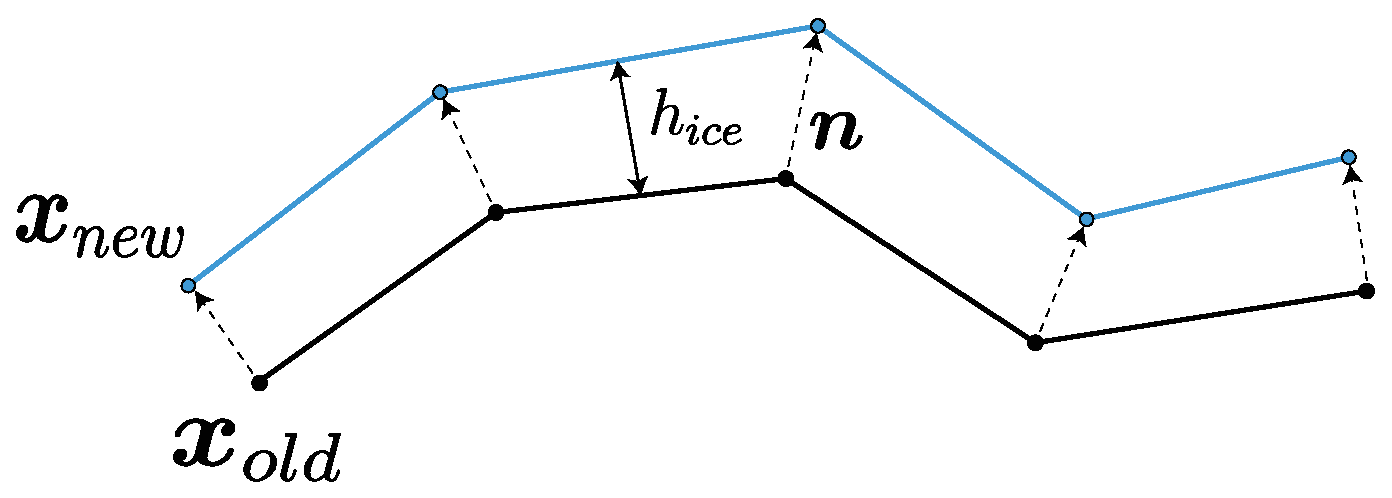
\includegraphics[width=\linewidth,height=2.05cm,keepaspectratio]{FIGURES/LEVELSET/LAGRANGIAN_NODE_DISPLACEMENT}
    \vspace{0.05cm}

    {\small
    \[
    \mathbf x_{\mathrm{new}}=\mathbf x_{\mathrm{old}}+
    h_{\mathrm{ice}}\mathbf n
    \]
    }
    \raggedright\small
    Surface nodes move along local normals, while the surrounding
    body-fitted mesh must be deformed or regenerated.
  \end{column}
  \hfill
  \begin{column}{0.53\textwidth}
    {\color{champsBlue}\bfseries Growing 3D Geometric Complexity}
    \vspace{0.10cm}

    \centering
    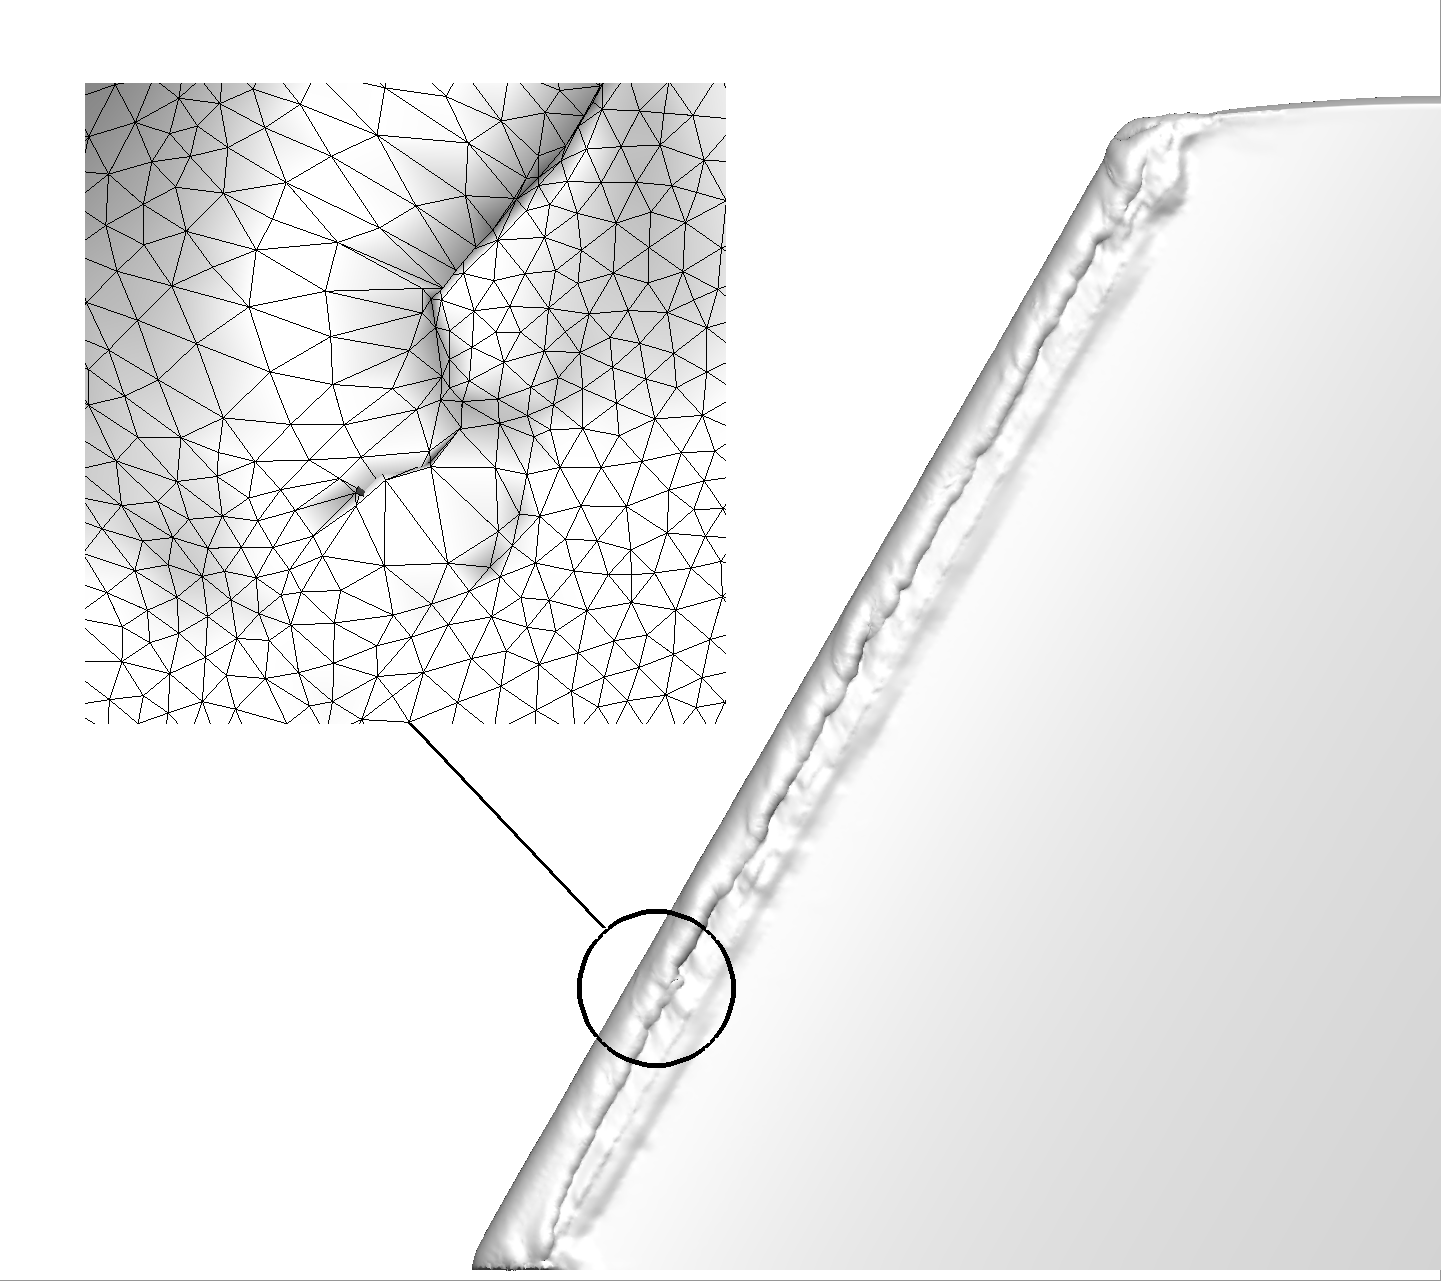
\includegraphics[width=\linewidth,height=3.65cm,keepaspectratio]{FIGURES/LEVELSET/ENTANGLEMENT.png}
    \vspace{0.03cm}

    {\scriptsize\color{gray}Surface-mesh distortion and entanglement near a 3D ice feature.}
    \vspace{0.08cm}

    \raggedright\small
    Horns, scallops, and concave regions may produce
    self-intersections or invalid elements.
  \end{column}
\end{columns}
\vfill
\begin{center}
  \colorbox{champsBlue!8}{\parbox{0.93\textwidth}{\centering\small
    \vspace{0.11cm}\textbf{Challenge:} Robust geometry evolution
    without preserving explicit surface-node connectivity.\vspace{0.11cm}}}
\end{center}
\end{frame}

% ---------------------------------------------------------------
% 2 — IMPLICIT SURFACE REPRESENTATION
% ---------------------------------------------------------------
\begin{frame}[t]{Implicit Interface Tracking: The Level-Set Method}
\vspace{0.12cm}
\begin{columns}[c,onlytextwidth]
  \begin{column}{0.40\textwidth}
    {\color{champsBlue}\bfseries Implicit Geometric Description}
    \vspace{0.15cm}

    \small
    The evolving ice--air boundary is represented by the
    \textbf{zero contour} of a signed-distance field $\phi$.
    \vspace{0.20cm}

    \[
    \boxed{\Gamma(t)=\{\mathbf x:\phi(\mathbf x,t)=0\}}
    \]

    \vspace{0.14cm}
    \begin{tabular}{@{}ll@{}}
      $\phi<0$ & Solid / ice\\[3pt]
      $\phi=0$ & Ice--air interface\\[3pt]
      $\phi>0$ & Air
    \end{tabular}
  \end{column}
  \hfill
  \begin{column}{0.58\textwidth}
    \centering
    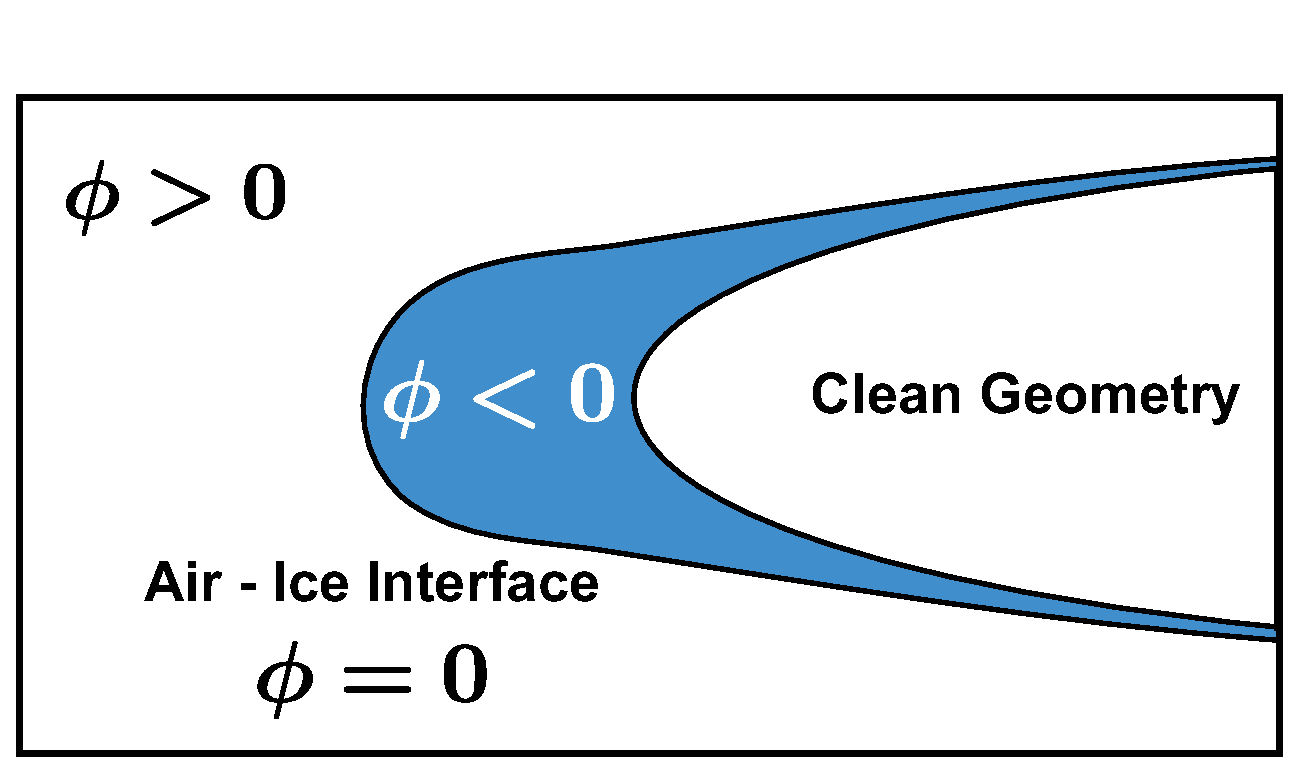
\includegraphics[width=\linewidth,height=3.68cm,keepaspectratio]{FIGURES/LEVELSET/ICE_AIR_INTERFACE}
  \end{column}
\end{columns}
\vspace{0.20cm}
\begin{center}
  {\color{champsBlue}\bfseries Evolve a field rather than moving surface nodes}
  \vspace{-0.13cm}
  \[
    \frac{\partial\phi}{\partial t}+\mathbf V\cdot\nabla\phi=0
  \]
\end{center}
\end{frame}

% ---------------------------------------------------------------
% 3 — NUMERICAL FORMULATION
% ---------------------------------------------------------------
\begin{frame}[t]{Level-Set Transport: Numerical Formulation}
\vspace{0.10cm}
\begin{center}
{\color{champsBlue}\bfseries Divergence form with a velocity-divergence correction}
\vspace{-0.13cm}
\[
\boxed{
\frac{\partial\phi}{\partial t}
+\nabla\cdot(\phi\mathbf V)
-\phi\,\nabla\cdot\mathbf V=0
}
\]
\end{center}
\vspace{-0.35cm}
\begin{columns}[T,onlytextwidth]
 \begin{column}{0.46\textwidth}
   {\color{champsBlue}\bfseries Ice-Growth Velocity}
   \vspace{-0.06cm}
   \[
     \mathbf V=\frac{h_{\mathrm{ice}}}{\Delta t_{\mathrm{layer}}}
     \mathbf n_{\phi_0},\qquad
     \mathbf n_{\phi_0}=\frac{\nabla\phi_0}{\lVert\nabla\phi_0\rVert}
   \]
   \vspace{0.08cm}
   \small
   Ice thickness is extended along the initial
   level-set normal direction, limiting redistancing needs
   for small layer displacements.
   \vspace{0.18cm}

   {\color{champsBlue}\bfseries Temporal Integration}
   \vspace{0.07cm}

   \small Semi-implicit \textbf{ROS22} (Rosenbrock--Wanner).
 \end{column}
 \hfill
 \begin{column}{0.50\textwidth}
   {\color{champsBlue}\bfseries Cell-Centered Finite Volumes}
   \vspace{-0.06cm}
   {\small
   \[
   \frac{\mathrm d\phi_i}{\mathrm dt}+R_i(\phi)=0
   \]
   \vspace{-0.17cm}
   \[
   R_i(\phi)=\frac{1}{|\Omega_i|}\sum_{f}
     (\phi_f-\phi_i)(\mathbf V_f\cdot\mathbf n_f)A_f
   \]
   }
   \vspace{0.04cm}
   \small
   \textbf{Spatial reconstruction:} second-order upwind;
   weighted least-squares gradients;
   Venkatakrishnan limiter.
 \end{column}
\end{columns}
\end{frame}

% ---------------------------------------------------------------
% 4 — INITIALIZATION AND SURFACE-VARIABLE EXTENSION
% ---------------------------------------------------------------
\begin{frame}[t]{Initialization and Extension of Surface Quantities}
\vspace{0.09cm}
\begin{columns}[T,onlytextwidth]
  \begin{column}{0.32\textwidth}
    \centering
    {\color{champsBlue}\bfseries Signed-Distance Initialization}
    \vspace{0.10cm}

    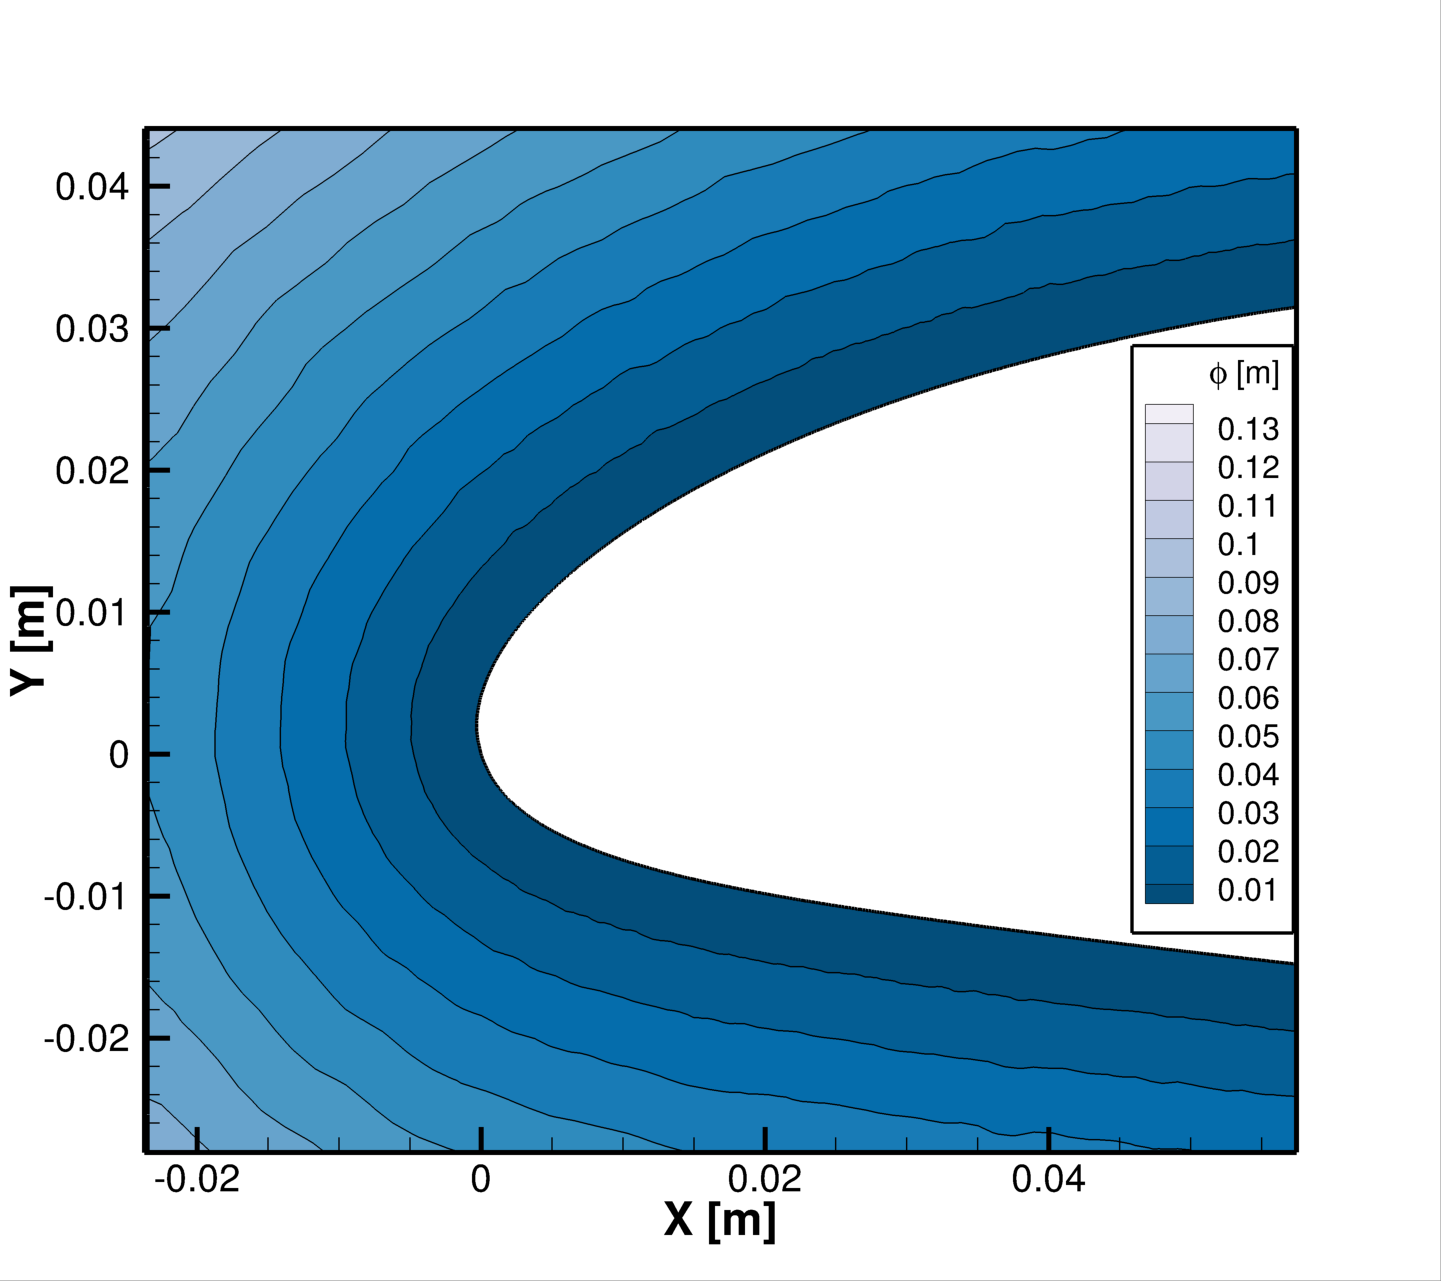
\includegraphics[width=\linewidth,height=2.28cm,keepaspectratio]{FIGURES/LEVELSET/EIKONAL.png}
    \vspace{-0.13cm}
    {\scriptsize
    \[
      \frac{\partial\phi}{\partial\tau}+
      \mathbf n_\phi\cdot\nabla\phi=1
    \]
    }
    \raggedright\scriptsize
    Eikonal pseudo-time transport with $\phi=0$ on the wall.
  \end{column}
  \hfill
  \begin{column}{0.32\textwidth}
    \centering
    {\color{champsBlue}\bfseries Ice-Thickness Extension}
    \vspace{0.10cm}

    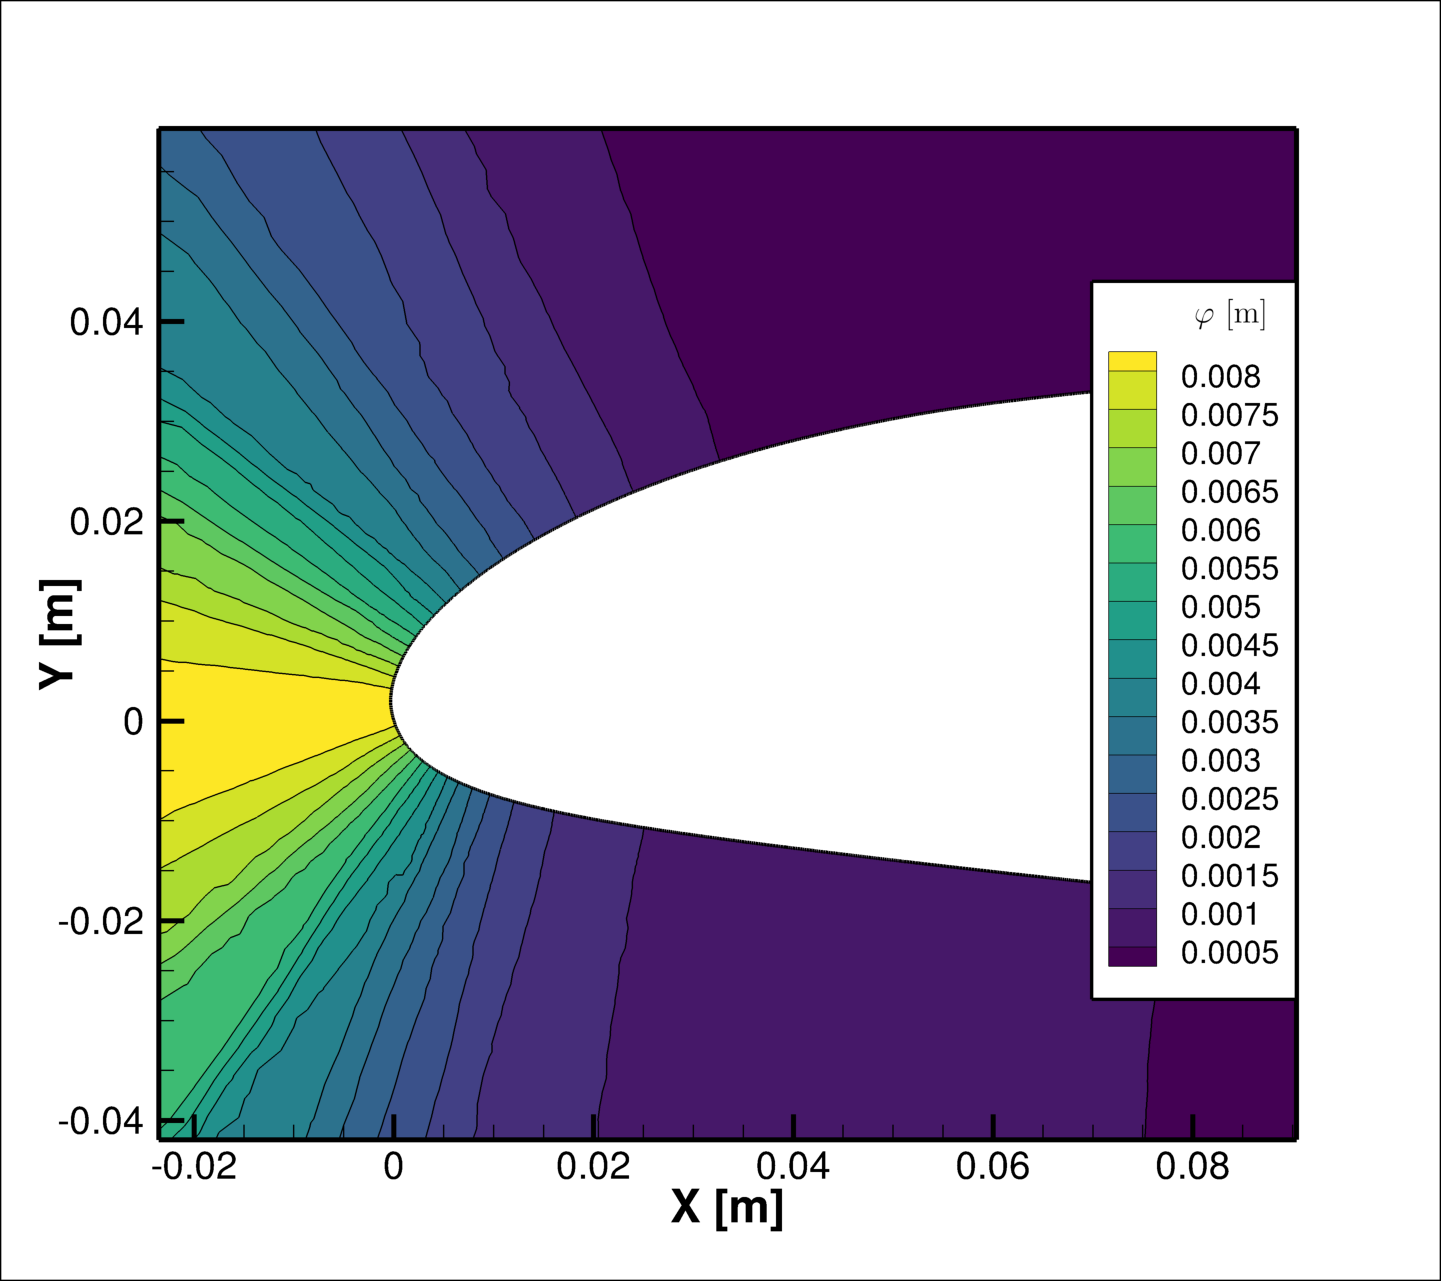
\includegraphics[width=\linewidth,height=2.28cm,keepaspectratio]{FIGURES/LEVELSET/PROPAGATION.png}
    \vspace{-0.13cm}
    {\scriptsize
    \[
      \frac{\partial\psi}{\partial\tau}+
      \mathbf n_\phi\cdot\nabla\psi=0
    \]
    }
    \raggedright\scriptsize
    Propagate surface ice thickness along signed-distance normals.
  \end{column}
  \hfill
  \begin{column}{0.32\textwidth}
    \centering
    {\color{champsBlue}\bfseries Geometric Alternative}
    \vspace{0.10cm}

    \FigOrPlaceholder{FIGURES/LEVELSET/AABB_TREE}{width=\linewidth,height=2.28cm,keepaspectratio}{2.0cm}
    \vspace{-0.13cm}
    {\scriptsize
    \[
      \phi(\mathbf x)=\pm\min_{T\in\Gamma}
      d(\mathbf x,T)
    \]
    }
    \raggedright\scriptsize
    Nearest-surface projection, accelerated by an AABB tree.
  \end{column}
\end{columns}
\vfill
\begin{center}
\colorbox{champsBlue!8}{\parbox{0.93\textwidth}{\centering\small
\vspace{0.10cm}
\textbf{Present framework:} Eikonal initialization and transport-based extension.
\quad\textbf{Alternative:} geometric closest-point projection with efficient spatial search.
\vspace{0.10cm}}}
\end{center}
\end{frame}

% ---------------------------------------------------------------
% 5 — MULTILAYER WORKFLOW
% ---------------------------------------------------------------
\begin{frame}[t]{CHAMPS -- Multilayer Ice-Accretion Approach}
\vspace{0.09cm}
\begin{columns}[T,onlytextwidth]
 \begin{column}{0.31\textwidth}
  \centering
  {\color{champsBlue}\bfseries 1. Icing Solution}
  \vspace{0.10cm}

  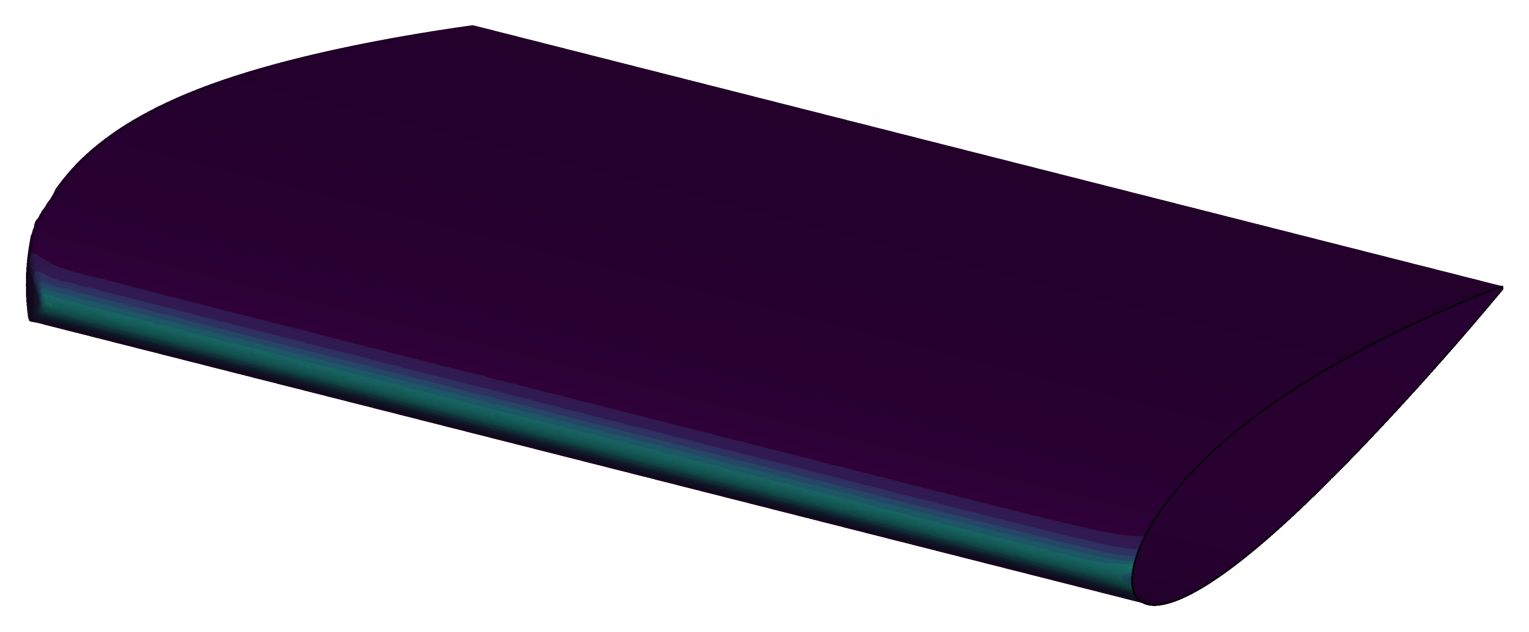
\includegraphics[width=\linewidth,height=2.40cm,keepaspectratio]{FIGURES/LEVELSET/THERMO_SOLUTION_CROP.png}
  \vspace{0.09cm}

  \raggedright\scriptsize
  \textbf{Flow $+$ droplets $+$ thermodynamics}
  \vspace{0.07cm}

  Obtain local ice mass accretion and thickness on the wing surface.
 \end{column}
 \hfill
 \begin{column}{0.31\textwidth}
  \centering
  {\color{champsBlue}\bfseries 2. Level-Set Evolution}
  \vspace{0.10cm}

  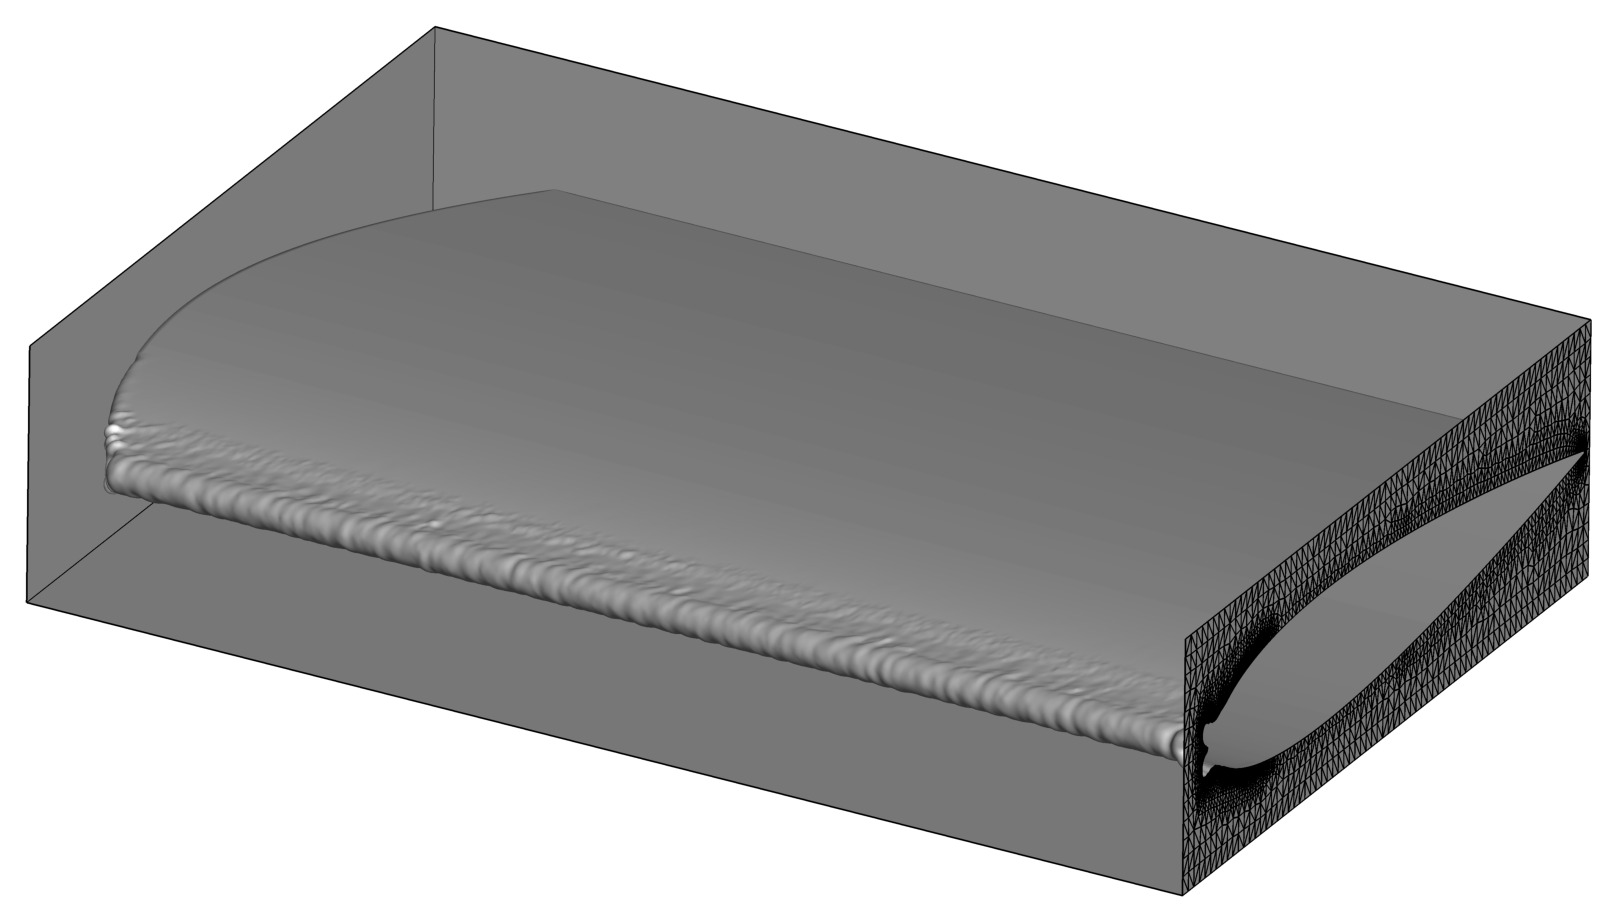
\includegraphics[width=\linewidth,height=2.40cm,keepaspectratio]{FIGURES/LEVELSET/LEVEL_SET_MESH_CROP.png}
  \vspace{0.09cm}

  \raggedright\scriptsize
  \textbf{Adapted auxiliary volume mesh}
  \vspace{0.07cm}

  $\sim$5--15 million cells; level-set transport $\sim$5 min per layer.
 \end{column}
 \hfill
 \begin{column}{0.31\textwidth}
  \centering
  {\color{champsBlue}\bfseries 3. Surface Reconstruction}
  \vspace{0.10cm}

  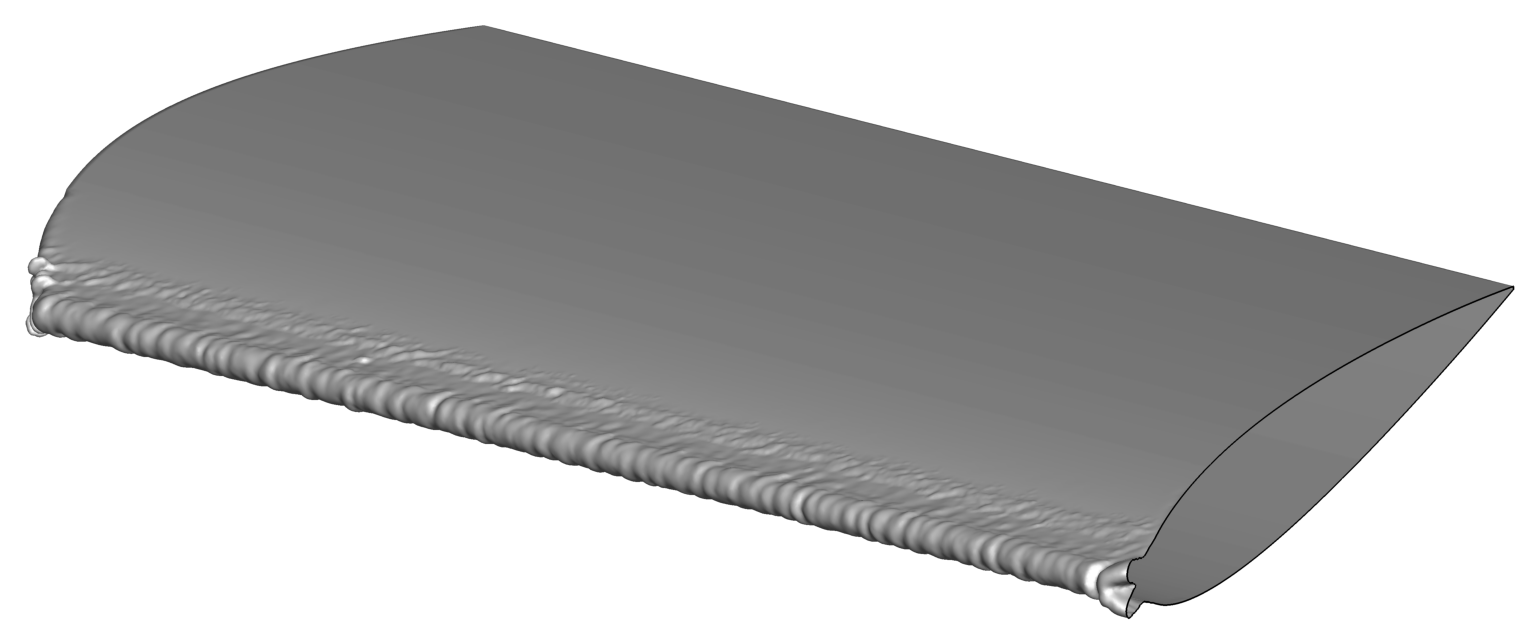
\includegraphics[width=\linewidth,height=2.40cm,keepaspectratio]{FIGURES/LEVELSET/LEVEL_SET_SURFACE_EXTRACTION_CROP.png}
  \vspace{0.09cm}

  \raggedright\scriptsize
  \textbf{MMG zero-isosurface extraction}
  \vspace{0.07cm}

  Surface smoothing and reconstruction; $\sim$20 min (serial bottleneck).
 \end{column}
\end{columns}
\vspace{0.32cm}
\begin{center}
\colorbox{champsBlue!8}{\parbox{0.92\textwidth}{\centering
\vspace{0.12cm}
{\color{champsBlue}\bfseries 4. Body-Fitted Volume Remeshing}
\vspace{0.07cm}

\small Automated Pointwise mesh update $\longrightarrow$
 recompute flow and impingement for the \textbf{next ice layer}.
\vspace{0.11cm}}}
\end{center}
\vfill
{\centering\tiny\color{gray}
Typical reported times vary with mesh size and workstation; 3D level set and extraction run locally.\par}
\end{frame}

% ---------------------------------------------------------------
% 6 — THREE-HORN BENCHMARK
% ---------------------------------------------------------------
\begin{frame}[t]{Three-Horn Benchmark: Geometry Robustness}
\vspace{0.13cm}
\begin{columns}[c,onlytextwidth]
 \begin{column}{0.64\textwidth}
  \centering
  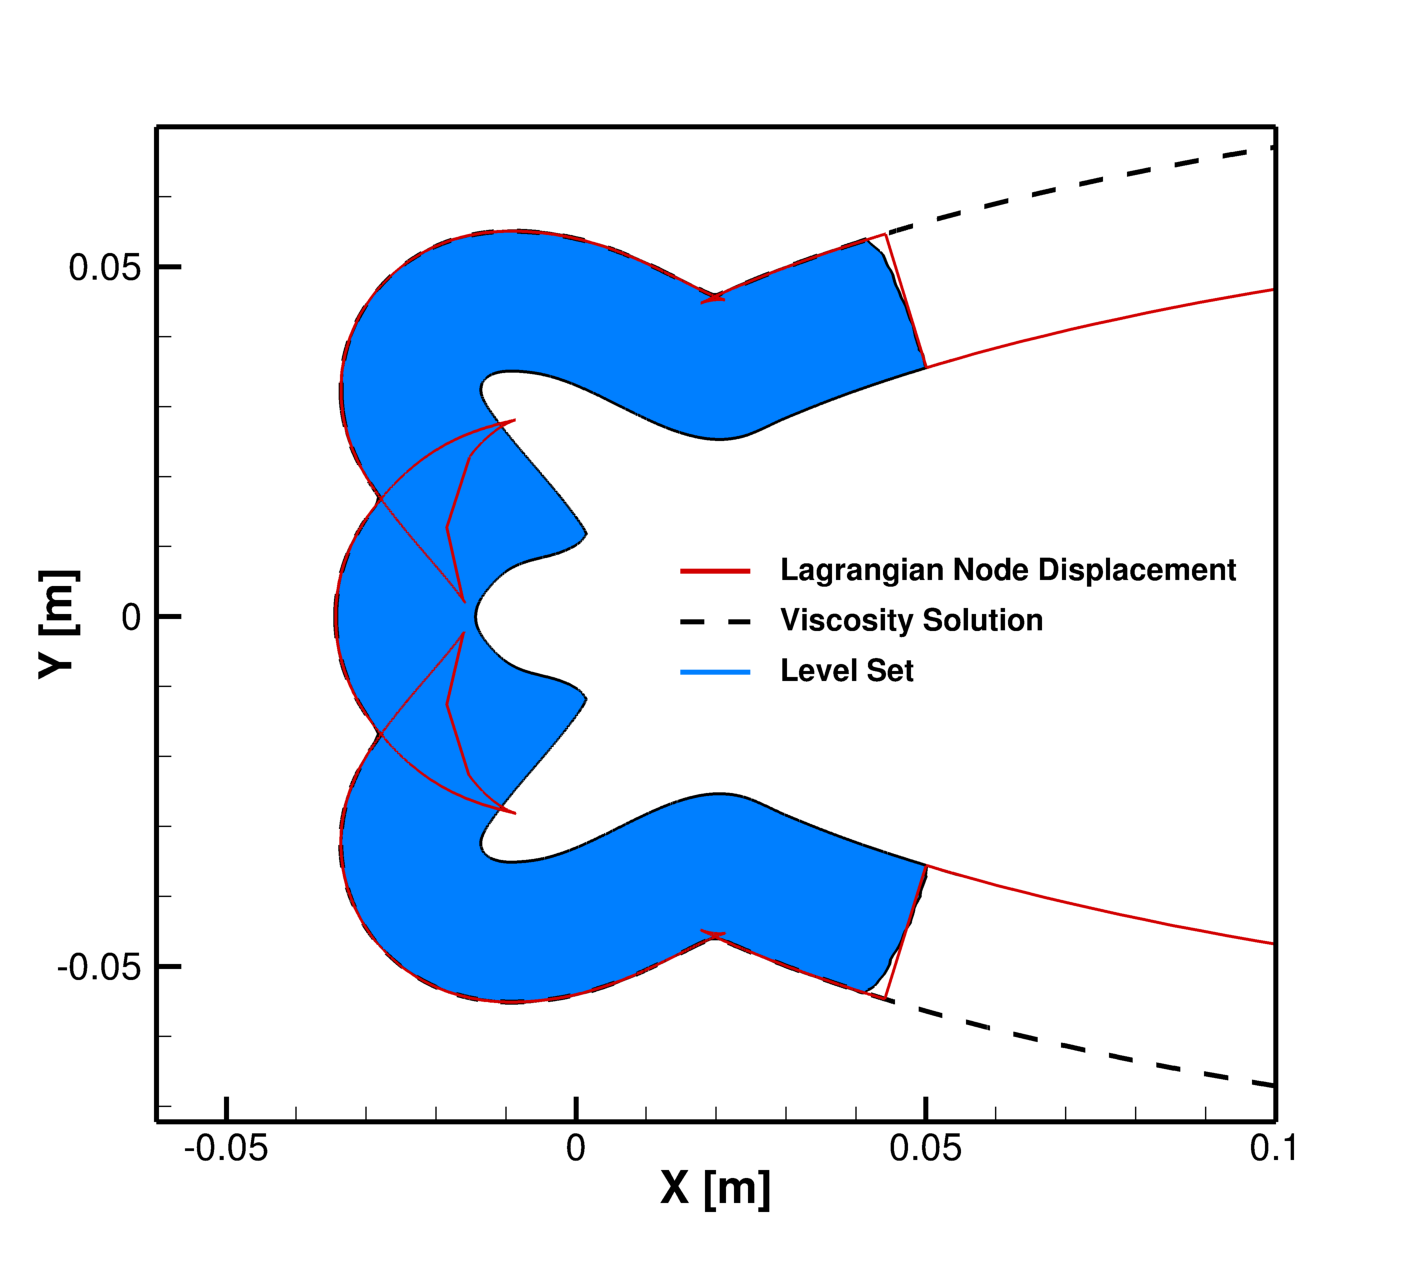
\includegraphics[width=\linewidth,height=5.00cm,keepaspectratio]{FIGURES/LEVELSET/THREE_HORNS.png}
 \end{column}
 \hfill
 \begin{column}{0.33\textwidth}
  {\color{champsBlue}\bfseries Manufactured Offset}
  \vspace{0.05cm}
  {\small\[
     h_{\mathrm{ice}}=0.02\,\mathrm m
     \qquad (x<0.05\,\mathrm m)
  \]}
  \vspace{0.13cm}
  {\color{red!75!black}\bfseries Direct Node Displacement}
  \vspace{0.06cm}
  \small Surface self-intersections and local ice-volume loss.
  \vspace{0.24cm}

  {\color{champsBlue}\bfseries Level-Set Evolution}
  \vspace{0.06cm}
  \small Reconstructs a valid front close to the exact geometric offset (viscosity solution).
 \end{column}
\end{columns}
\vfill
\begin{center}
\colorbox{champsBlue!8}{\parbox{0.92\textwidth}{\centering\small
\vspace{0.10cm}Implicit evolution handles concave, merging ice features without explicit surface entanglement.
\vspace{0.10cm}}}
\end{center}
\end{frame}

% ---------------------------------------------------------------
% 7 — IPW1 CASE 362: THREE-DIMENSIONAL MORPHOLOGY
% ---------------------------------------------------------------
\begin{frame}[t]{IPW1 Case 362: Three-Dimensional Scallop Formation}
\vspace{0.05cm}
{\centering\scriptsize
30$^\circ$ swept NACA 0012 \; $\vert$ \;
$T_\infty=266$ K \; $\vert$ \; 20 min icing \; $\vert$ \;
10 accretion layers
\par}
\vspace{0.10cm}
\begin{columns}[c,onlytextwidth]
  \begin{column}{0.42\textwidth}
    \centering
    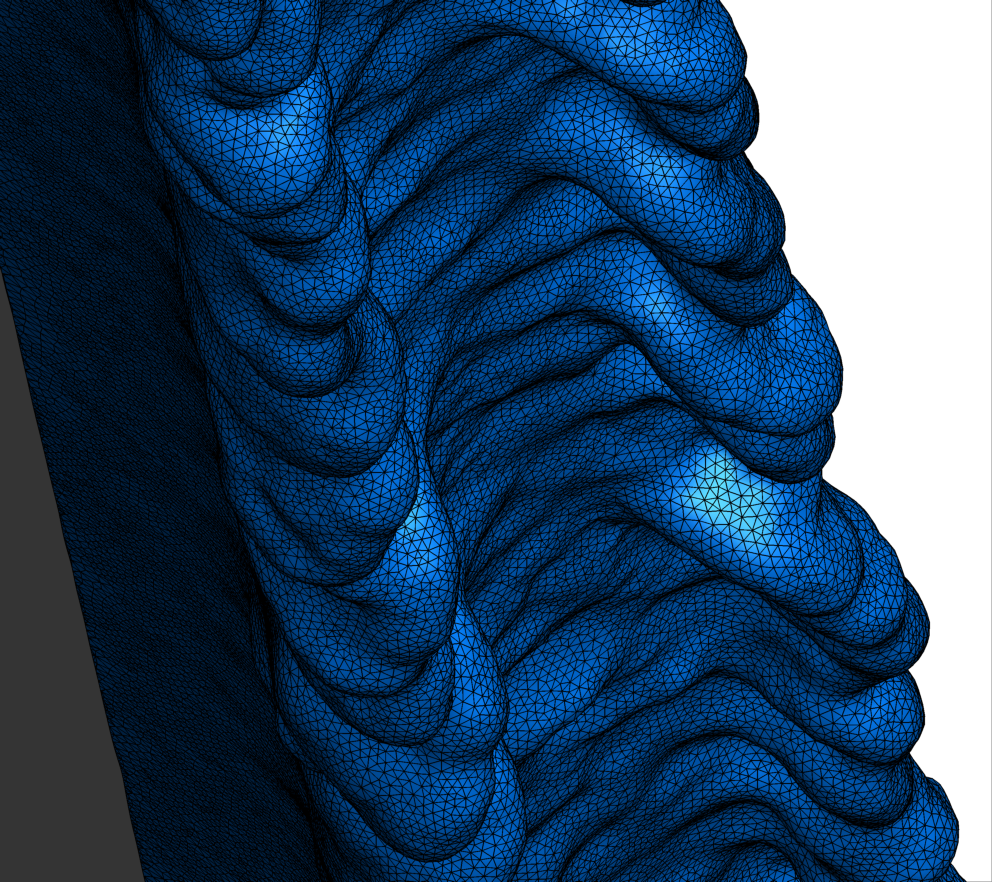
\includegraphics[width=\linewidth,height=4.40cm,keepaspectratio]{FIGURES/LEVELSET/CLIPPED_ICE_SHAPE_CASE_362_3.png}\par
    \vspace{0.04cm}
    {\scriptsize\color{gray}Scallops and adapted surface mesh.}
  \end{column}
  \hfill
  \begin{column}{0.55\textwidth}
    \centering
    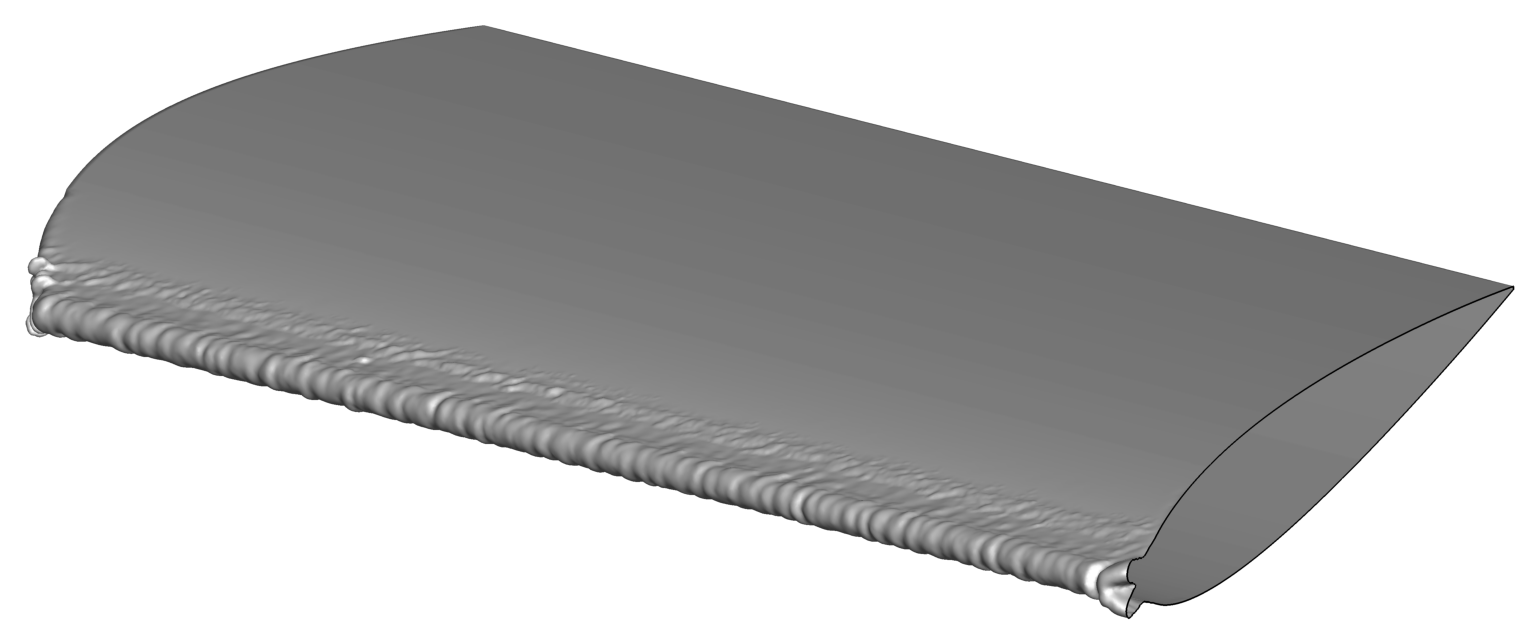
\includegraphics[width=\linewidth,height=4.30cm,keepaspectratio]{FIGURES/LEVELSET/LEVEL_SET_SURFACE_EXTRACTION_CROP.png}\par
    \vspace{0.04cm}
    {\scriptsize\color{gray}Reconstructed three-dimensional ice geometry.}
  \end{column}
\end{columns}
\vfill
\begin{center}
\colorbox{champsBlue!8}{\parbox{0.93\textwidth}{\centering\small
\vspace{0.11cm}Multilayer level-set evolution captures complex
spanwise ice features while maintaining a conformal extracted surface.
\vspace{0.11cm}}}
\end{center}
\end{frame}

% ---------------------------------------------------------------
% 8 — IPW1 CASE 362: CROSS SECTION / EXPERIMENT
% ---------------------------------------------------------------
\begin{frame}[t]{IPW1 Case 362: Ice-Shape Comparison}
\vspace{0.07cm}
{\centering\scriptsize
30$^\circ$ swept NACA 0012 \; $\vert$ \;
LWC = 0.5 g/m$^3$ \; $\vert$ \;
MVD = 34.7 $\mu$m \; $\vert$ \;
$k_s/c=0.001$
\par}
\vspace{0.14cm}
\begin{columns}[c,onlytextwidth]
  \begin{column}{0.65\textwidth}
    \centering
    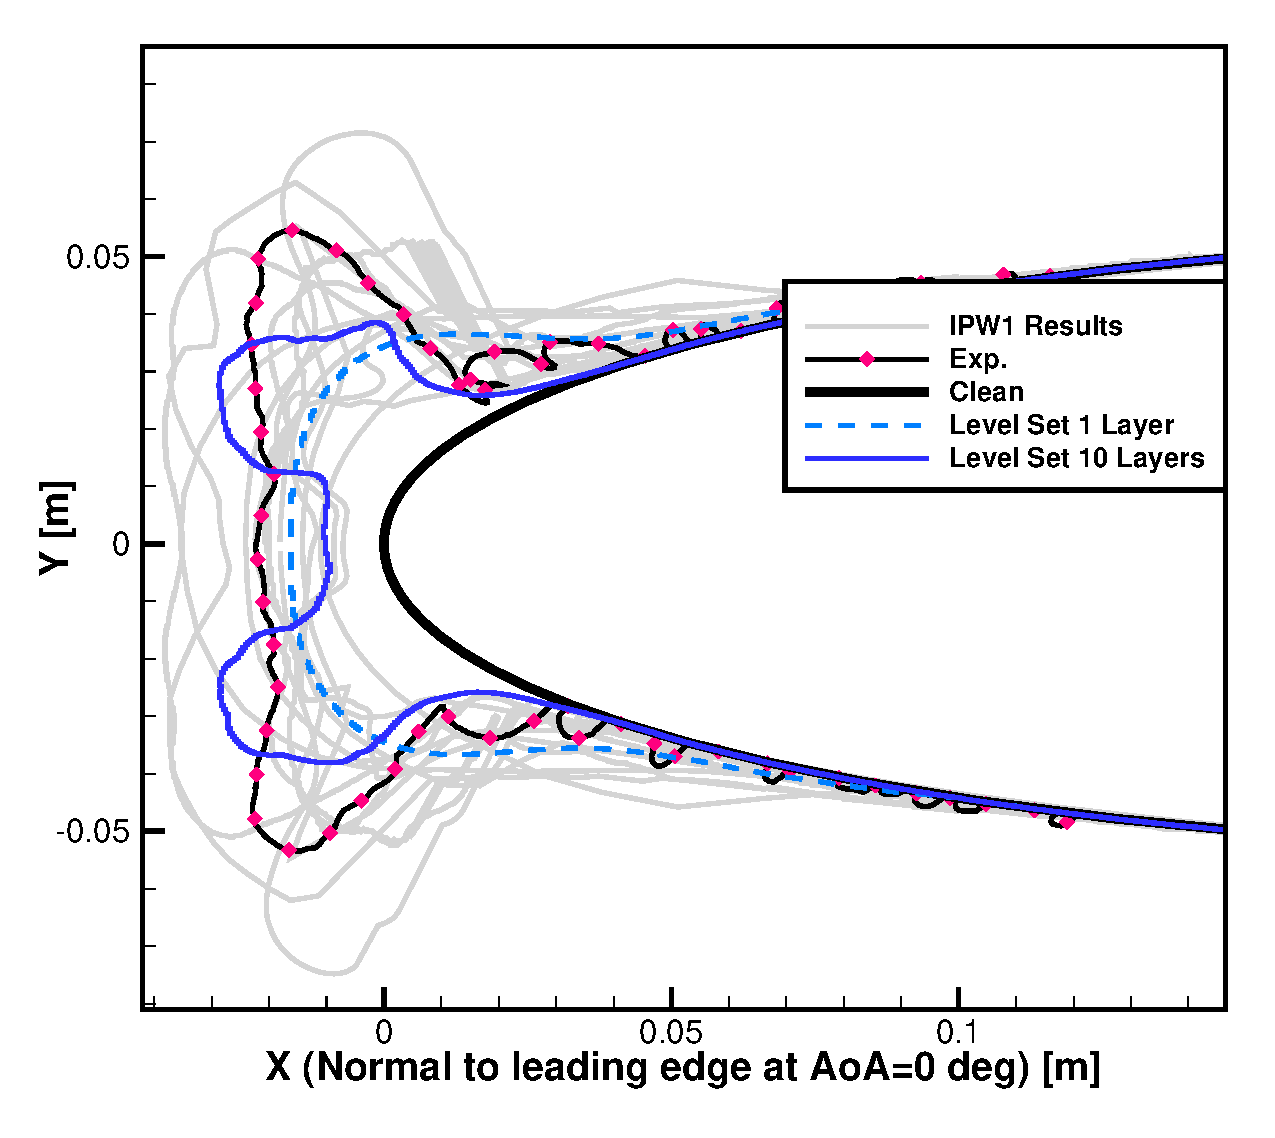
\includegraphics[width=\linewidth,height=4.82cm,keepaspectratio]{FIGURES/LEVELSET/CASE_IPW1_362_ICE_SHAPE}
  \end{column}
  \hfill
  \begin{column}{0.32\textwidth}
    {\color{champsBlue}\bfseries Single Step vs. 10 Layers}
    \vspace{0.10cm}

    \small Multilayer predictions reproduce horn and scallop development
    not captured in one step.
    \vspace{0.30cm}

    {\color{champsBlue}\bfseries Experimental Comparison}
    \vspace{0.10cm}

    \small Reasonably good overall agreement of the
    maximum combined cross section (MCCS).
    \vspace{0.25cm}

    {\color{red!70!black}\bfseries Remaining Discrepancies}
    \vspace{0.10cm}

    \small Horn orientation and impingement limits.
  \end{column}
\end{columns}
\vfill
\begin{center}
\colorbox{champsBlue!8}{\parbox{0.92\textwidth}{\centering\small
\vspace{0.10cm}2D MCCS comparisons do not fully reveal the local spanwise variation
of genuinely three-dimensional ice structures.\vspace{0.10cm}}}
\end{center}
\end{frame}

